%% Submissions for peer-review must enable line-numbering
%% using the lineno option in the \documentclass command.
%%
%% Preprints and camera-ready submissions do not need
%% line numbers, and should have this option removed.
%%
%% Please note that the line numbering option requires
%% version 1.1 or newer of the wlpeerj.cls file, and
%% the corresponding author info requires v1.2

\documentclass[fleqn,10pt]{wlpeerj} % for preprint submissions

% ZNK -- Adding headers for pandoc

\setlength{\emergencystretch}{3em}
\providecommand{\tightlist}{
\setlength{\itemsep}{0pt}\setlength{\parskip}{0pt}}
\usepackage{lipsum}
\usepackage[unicode=true]{hyperref}
\usepackage{longtable}



\usepackage{lipsum} \usepackage{float}

\title{Juvenile Salmon Migration Observations in the Discovery Islands and
Johnstone Strait in 2018}

\author[1]{Brett T. Johnson}

\corrauthor[1]{Brett T. Johnson}{\href{mailto:brett.johnson@hakai.org}{\nolinkurl{brett.johnson@hakai.org}}}
\author[]{Julian C.L. Gan}

\author[]{Carly V. Janusson}

\author[1, 2, 3]{Brian P.V. Hunt}


\affil[1]{Hakai Institute Quadra Island Ecological Observatory, Heriot Bay, BC V0P
1H0}
\affil[2]{Institute for the Oceans and Fisheries, University of British Columbia
Vancouver, B.C., Canada V6T 1Z4}
\affil[3]{Department of Earth, Ocean and Atmospheric Sciences, University of
British Columbia Vancouver, B.C., Canada V6T 1Z4}


%
% \author[1]{First Author}
% \author[2]{Second Author}
% \affil[1]{Address of first author}
% \affil[2]{Address of second author}
% \corrauthor[1]{First Author}{f.author@email.com}

% 


\begin{abstract}
The majority of out-migrating juvenile Fraser River sockeye
(\emph{Oncorhynchus} \emph{nerka}), pink (\emph{O.} \emph{gorbuscha}),
and chum (\emph{O.} \emph{keta}) salmon pass northwest through the
Strait of Georgia, the Discovery Islands, and Johnstone Strait. The
Discovery Islands to Johnstone Strait leg of the migration is a region
of poor survival for juvenile salmon relative to the Strait of Georgia.
To better understand the factors that are driving early marine survival
through this region the Hakai Institute Juvenile Salmon Program monitors
key aspects of this migration. Here we report on the 2018 migration in
comparison to averages from the 2015--2018 study period. In 2018
sockeye, pink, and chum migration timing was not significantly different
than time series averages. The median capture date in the Discovery
Islands was May 23rd for sockeye, and June 12th for pink and chum. Pink
salmon had the highest catch proportion and the highest average catch
intensity in 2018 followed by chum and sockeye. Sockeye were longer than
average in 2018 whereas pink and chum were smaller than average (all
\emph{p} \textless{} 0.001). In the Discovery Islands sea lice abundance
was lower than average for sockeye, pink, and chum. In Johnstone Strait
sea lice abundance was lower for chum but higher than average for
sockeye and pink. Notably, there were no \emph{Lepeophtheirus salmonis}
sea lice observed in Johnstone Strait in 2018. Sea surface temperatures
in the northern Strait of Georgia during the smolt migration period of
2018 were the warmest on record in the study period.
% Dummy abstract text. Dummy abstract text. Dummy abstract text. Dummy abstract text. Dummy abstract text. Dummy abstract text. Dummy abstract text. Dummy abstract text. Dummy abstract text. Dummy abstract text. Dummy abstract text.
\end{abstract}

\begin{document}

\flushbottom
\maketitle
\thispagestyle{empty}

\section{Introduction}\label{introduction}

The first months after marine entry have been identified as a
potentially critical period (Beamish and Mahnken 2001) for salmon stock
recruitment, which may ultimately be responsible for inter-annual
variability and long term declines in salmon stocks in British Columbia
(Peterman et al. 2010; Beamish et al. 2012). Pathogens, parasites,
predators and the impacts of climate change on food web dynamics have
emerged as leading causes for the decline. The Hakai Institute Juvenile
Salmon Program has been monitoring juvenile salmon migrations in the
Discovery Islands and Johnstone Strait (Figure \ref{fig:map}) since 2015
in an effort to understand what factors may be influencing early marine
survival of sockeye, pink, and chum (Hunt et al. 2018). This report
summarizes migration timing, fish length, parasite loads, species
composition, and sea-surface temperature observed from the first 4 years
of this research and monitoring program. These estimates will provide
the context from which to investigate questions and interpret results
related to growth, survival, and the conditions salmon experience during
their migration through this critical region.

\begin{figure}[H]

\includegraphics[width=0.9\linewidth]{map} \hfill{}

\caption{Sampling locations in 2018}\label{fig:map}
\end{figure}

\section{Methods}\label{methods}

\subsection{Field methods}\label{field-methods}

See Hunt et al. (2018) for a detailed description of field and lab
methods. Briefly, juvenile salmon were collected weekly from the
Discovery Islands and Johnstone Strait during their northward migration
from the Strait of Georgia to Queen Charlotte Strait near northern
Vancouver Island, British Columbia. Sampling was conducted from May to
July each year beginning in 2015 using purse seine nets (bunt: 27 m x 9
m with 13 mm mesh; tow: 46 m x 9 m with 76 mm mesh). Near shore marine
habitats where depth was \textgreater{} 10 m were sampled and sockeye
(\emph{Oncorhynchus nerka}), pink (\emph{O. gorbuscha}), chum (\emph{O.
keta}) were effectively sampled and coho (\emph{O. kisutch}), Chinook
(\emph{O. tshawytschya}) and Pacific herring (\emph{Clupea pallasii})
were incidentally captured. All animal care was in accordance with
Animal Care Guidelines under permit A16-0101. Temperature data were
collected by deploying an RBR conductivity, temperature, and depth
profiler to depths \textgreater{} 30 m at station QU39 (Figure
\ref{fig:map}) in the northern Strait of Georgia.

\subsection{Data Analysis}\label{data-analysis}

Time series anomalies reported are in relation to the time series
averages (2015-2018). The mean for each parameter of interest was
calculated for all years combined, and the z-score was calculated for
each parameter to determine the number of standard deviations away from
the mean a given parameter was in each year. Measurements from the
Discovery Islands and Johnstone Strait regions of the salmon migration
were combined in analyses unless otherwise indicated. All analyses were
conducted using R (R Core Team 2017).

The peak migration date for each species was estimated by calculating
the median date of capture in the Discovery Islands. This method was
used because the period in which surveys and seines were conducted was
the same each year and seines were always conducted before sockeye
arrived and after sockeye disappeared. Often, however, the entire
duration of the pink and chum migration through the Discovery Islands
was not captured because their migration period is more protracted
compared to sockeye. Cumulative abundance was calculated over a
constrained period between May 1st and July 9th of each year. Seines
from Johnstone Strait were excluded from the migration timing
calculation so that timing indicates the migration through the Discovery
Islands. Because very few pink are caught in odd-years, only even-years
were included in the calculation of the pink time series average.

Catch intensity was calculated to provide a measure of inter-annual
abundance for sockeye, pink, and chum. Catch intensity was defined as
the average number of fish captured when greater than 1 sockeye was
caught. In effect, catch intensity summarizes the abundance of each
species in a community of co-migrating sockeye, pink, and chum when
sockeye are always present.

Species proportions were calculated by dividing the total number of each
species caught, by the sum of all species caught that season. Only
seines that caught sockeye were used in the calculation of species to
represent the salmon community composition that co-migrate with sockeye.
To test whether fork lengths from 2018 were significantly different than
the time series an independent two-group t-test was conducted. Fork
length distributions were visualized by calculating length frequency
distributions using kernel density estimates from fork length data.

The prevalence, intensity, and abundance of \emph{Caligus clemensi} and
\emph{Lepeophtheirus salmonis} sea lice parasites were calculated
according to the definitions in Margolis et al. (1990). Naplius and
chalimus life stages were not included in our analyses, only adult
motile stages were analyzed. So few \emph{L. salmonis} sea lice were
observed that their counts were combined with \emph{C. clemensi} and
combined species parasite loads are reported.

The mean sea surface temperature (SST) was calculated from the top 30 m
of the water column in May and June---the period during which salmon
migrate through the region. To visualize temperature anomalies, a loess
regression was applied to sea surface temperatures from all years to
develop a model that represents the average seasonal trend. Deviations
above or below the seasonal trend were coloured red or blue respectively
to indicate the direction and magnitude of the anomaly.

\section{Results and Discussion}\label{results-and-discussion}

Most migration parameters were below average in 2018 except for sockeye
length and SST (Figure \ref{fig:heatmap}). Interestingly, sockeye length
tends to be the opposite anomaly compared to pink and chum which vary
together.

Migration timing in the Discovery Islands in 2018 did not differ from
the time series average by more than a week for sockeye, pink, or chum
(Figure \ref{fig:mt}) (Table \ref{tab:mtdi}). The peak migration date
for sockeye in the Discovery Islands was on May 23, 5 days earlier than
the time series average of May 28. The peak migration date for pink in
the Discovery Islands was on June 12, 5 days earlier than the average of
June 17. The peak migration date for chum in the Discovery Islands was
on June 12, 3 days earlier than the average of June 15.

Sockeye catch intensity in 2018 was low relative to sockeye in previous
years and relative to pink and chum in 2018 (Figure
\ref{fig:catchintensity}). That sockeye catch intensity was low in 2018
is not surprising because 2016 brood year Shuswap or Chilko Lake sockeye
are not as abundant in this cohort as they are in others. Pink catch
intensity in 2018 was the highest of the four years measured. Pink
out-migrants are more abundant on even years, the result of the odd-year
dominant life-cycle of Fraser River pinks (Heard 1991), but 2018 catches
indicate either good production or good survival in the early marine
environment for pink salmon relative to 2016---the only other odd-year
dominant brood year recorded by the Juvenile Salmon Program.

Pink salmon dominated the catch in the Discovery Islands and Johnstone
in 2018 making up 51.9 \% of the catch (Table \ref{tab:proptable}) while
chum made up 32.4 \% and sockeye 12.9 \% (Figure \ref{fig:prop}). This
was the first time in the time series that pink dominated the catch
proportion.

Fish lengths varied between regions, species and year (Figure
\ref{fig:lengthplot}) though in 2018 sockeye were longer, pink were
shorter, and chum were shorter than their respective time series
averages in the Discovery Islands and Johnstone Strait combined. Sockeye
length was 116.9 mm (Table \ref{tab:length}), which is 8.9 mm longer
than the time series average (\emph{p} \textless{} 0.0001, 95\% CI 6.2
--11.7). Average pink lengths were 96.3 mm, which is 8.8 mm shorter than
the time series average (\emph{p} \textless{} 0.0001, 95\% CI
10.9--6.7). Chum were on average 103.4 mm, which is 7 mm shorter than
the time series average (\emph{p} \textless{} 0.0001, 95\% CI 8.9---5).

The abundance of motile sea lice in 2018 was the among the lowest
recorded in the Discovery Islands time-series while Johnstone Strait
parasite loads were average. (Figure \ref{fig:parasites}). Notably, no
\emph{Lepeophtheirus salmonis} were detected on sockeye in Johnstone
Strait, despite being present in the Discovery Islands. Pink salmon had
higher sea lice abundance, prevalence, and intensity compared to the
chum and sockeye time series average (Table \ref{tab:sealice}) in
contrast to Patanasatienkul et al. (2013) where they found that the
prevalence and intensity of sea lice was higher on chum than pink on
early marine entrants in the Broughton Archipelago.

Sea-surface temperature in May and June during the juvenile salmon
out-migration at QU39 in the northern Strait of Georgia was 0.39 degrees
C warmer than average (Table \ref{tab:ssttable}) (Figure \ref{fig:sst}).
In the context of the last four last years 2018 was the warmest surface
waters observed in the northern Strait of Georgia, despite 2015 SST
along the BC coast breaking records for high temperatures (Chandler,
King, and Boldt 2017).

\begin{figure}[H]
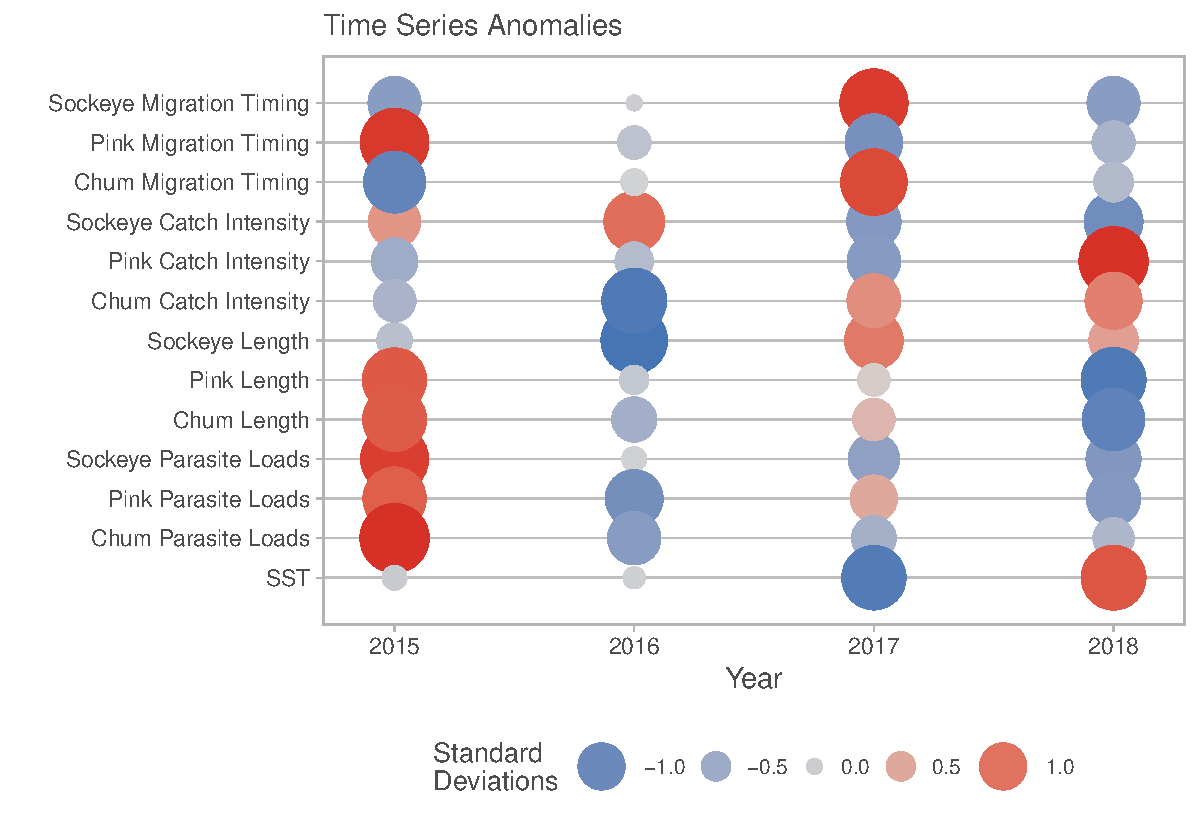
\includegraphics[width=0.95\linewidth]{Migration_Observations_Report_files/figure-latex/heatmap-1} \caption{This heatmap indicates the number of standard deviations (z-score) from the time series average (2015-2018) for key migration parameters. Blue colour indicates less than average, grey indicates average, red indicates greater than average. Peak migration date is based on the median date of fish capture in the Discovery Islands. Length is based on the average fork length from the the Discovery Islands and Johnstone Strait combined. Parasite load is the average abundance of all sea lice species in their motile life stage for both the Discovery Islands and Johnstone Strait regions combined. Mean sea-surface temperature is 30 m depth integrated temperature from station QU39 in the Northern Strait of Georgia from May and June.}\label{fig:heatmap}
\end{figure}

\begin{figure}[H]
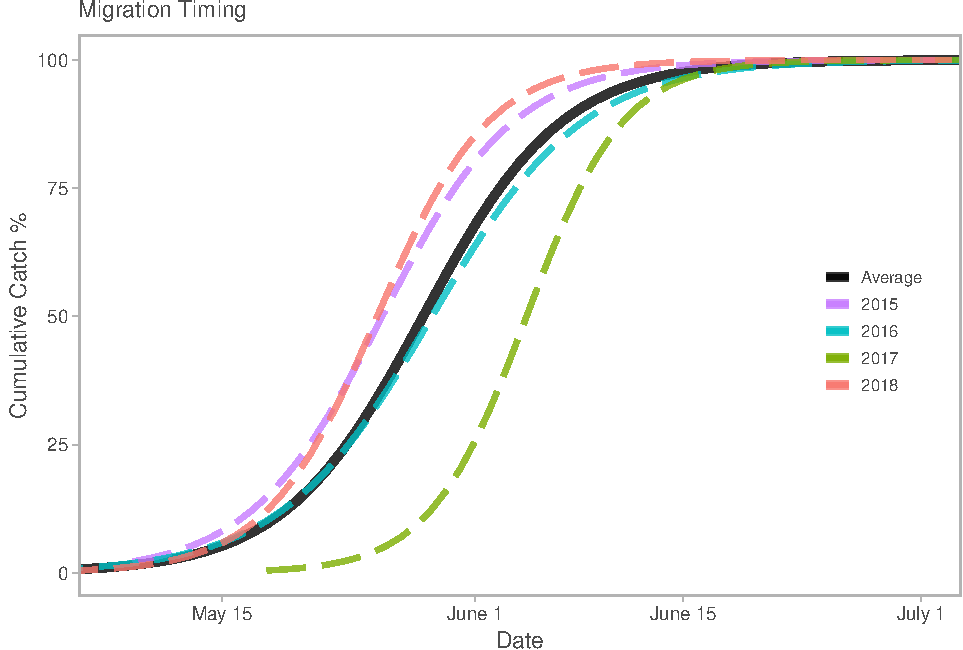
\includegraphics[width=0.9\linewidth]{Migration_Observations_Report_files/figure-latex/mt-1} \caption{Cumulative abundance of sockeye, pink, and chum caught in the Discovery Islands and Johnstone Strait compared to the time series average.}\label{fig:mt}
\end{figure}

\begin{figure}[H]
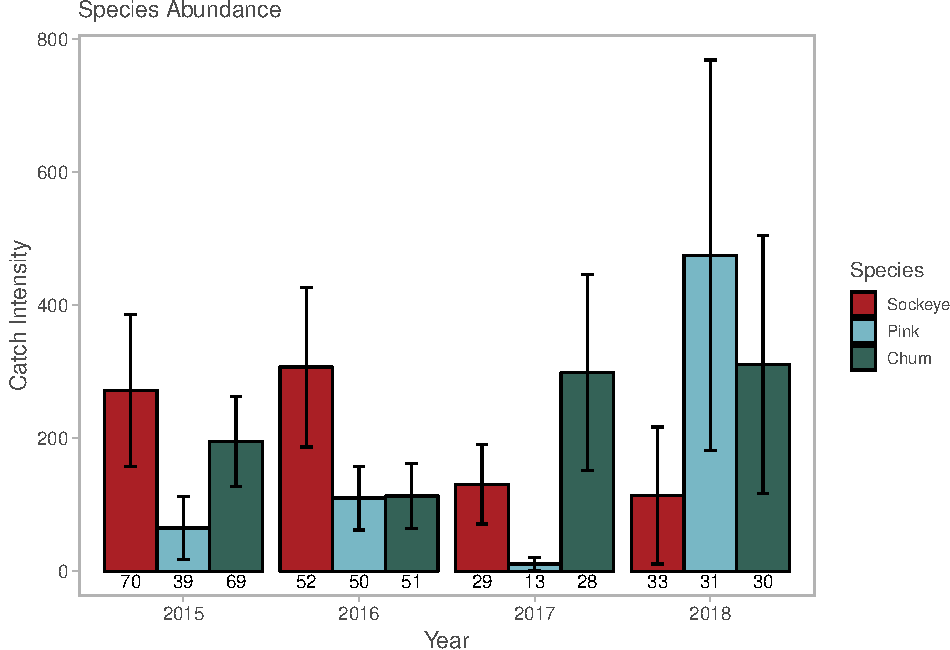
\includegraphics[width=0.9\linewidth]{Migration_Observations_Report_files/figure-latex/catchintensity-1} \caption{The catch intensity (a measure of abundance) of sockeye, pink, and chum salmon in the Discovery Islands and Johnstone Strait. Numbers under each bar indicate the number of seines in which the species was caught, and erorr bars indicate the 95 percent confidence region.}\label{fig:catchintensity}
\end{figure}

\begin{figure}[H]
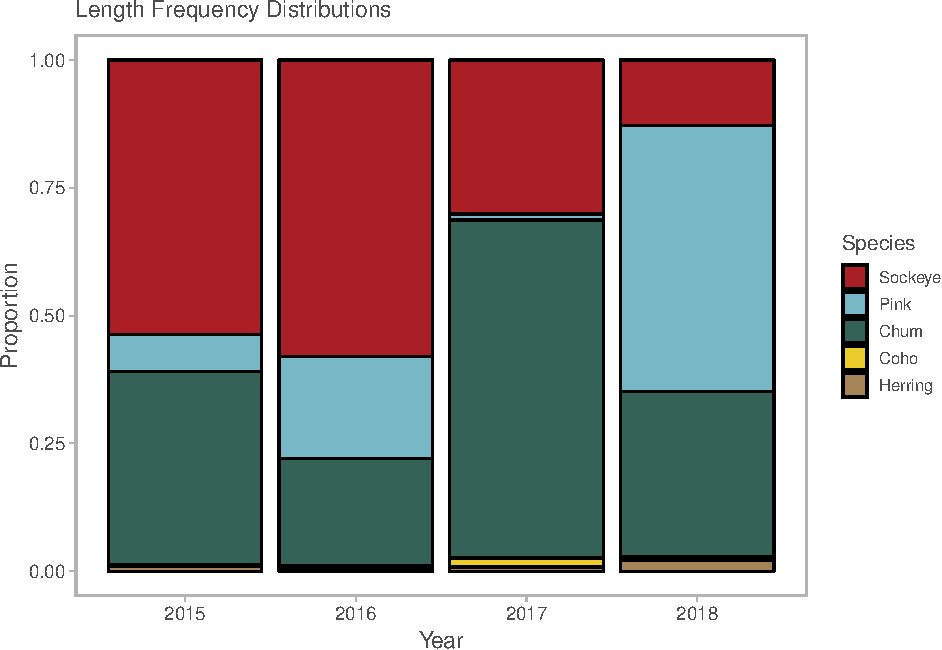
\includegraphics[width=0.9\linewidth]{Migration_Observations_Report_files/figure-latex/prop-1} \caption{The annual proportion of fish captured in the Discovery Islands and Johnstone Strait combined.}\label{fig:prop}
\end{figure}

\begin{figure}[H]
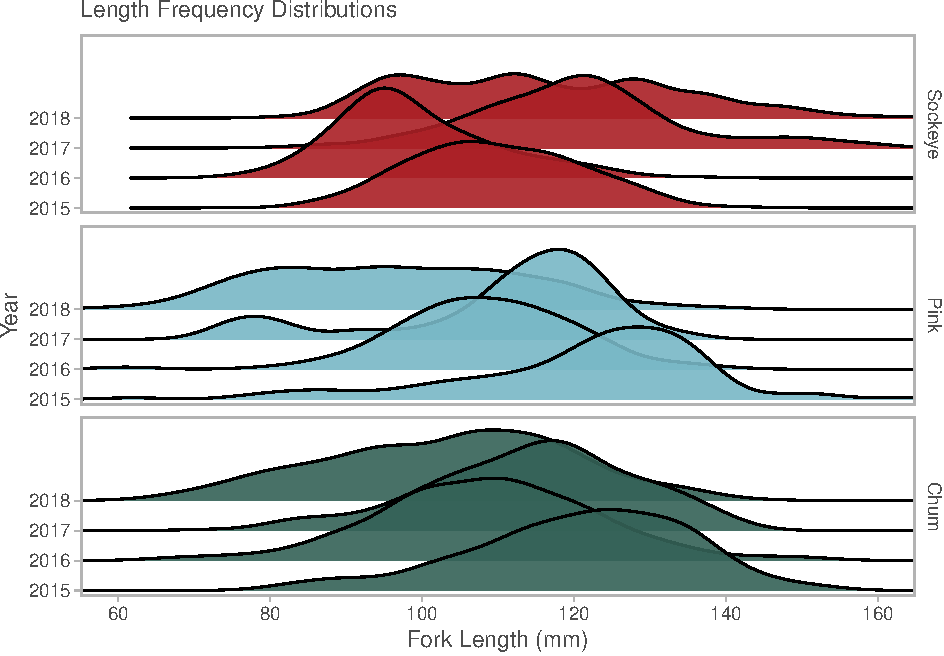
\includegraphics[width=0.9\linewidth]{Migration_Observations_Report_files/figure-latex/lengthplot-1} \caption{Distributions of juvenile salmon fork lengths for each year in the Discovery Islands and Johnstone Strait. Note that these distributions contain multiple age-classes.}\label{fig:lengthplot}
\end{figure}

\begin{figure}[H]
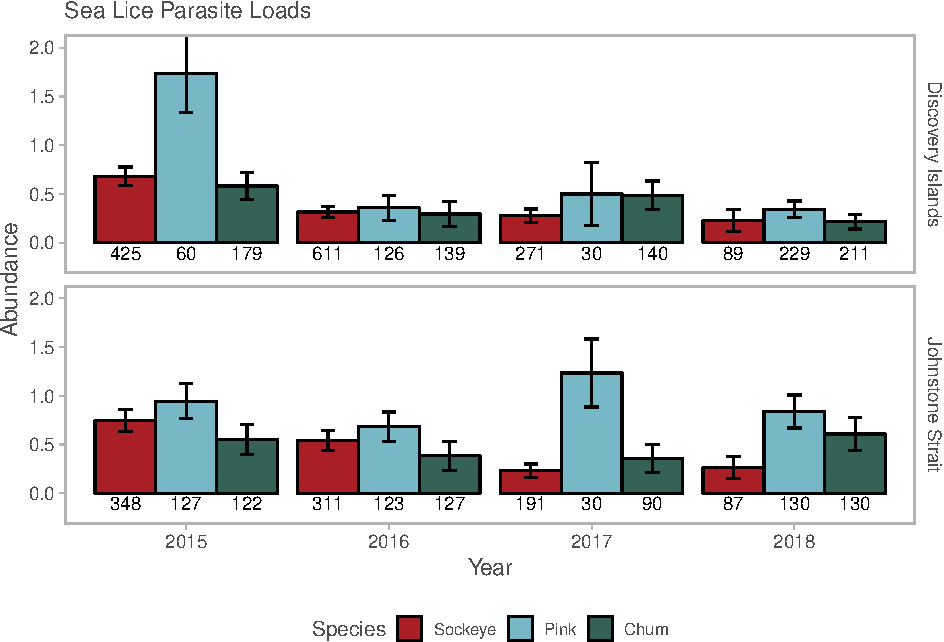
\includegraphics[width=0.9\linewidth]{Migration_Observations_Report_files/figure-latex/sealice-1} \caption{The abundance of motile sea lice on juvenile salmon in the Discovery Islands and Johnstone Strait. The numbers under each bar indicate the sample size and the error bars indicate the 95 percent confidence region.}\label{fig:sealice}
\end{figure}

\begin{figure}[H]
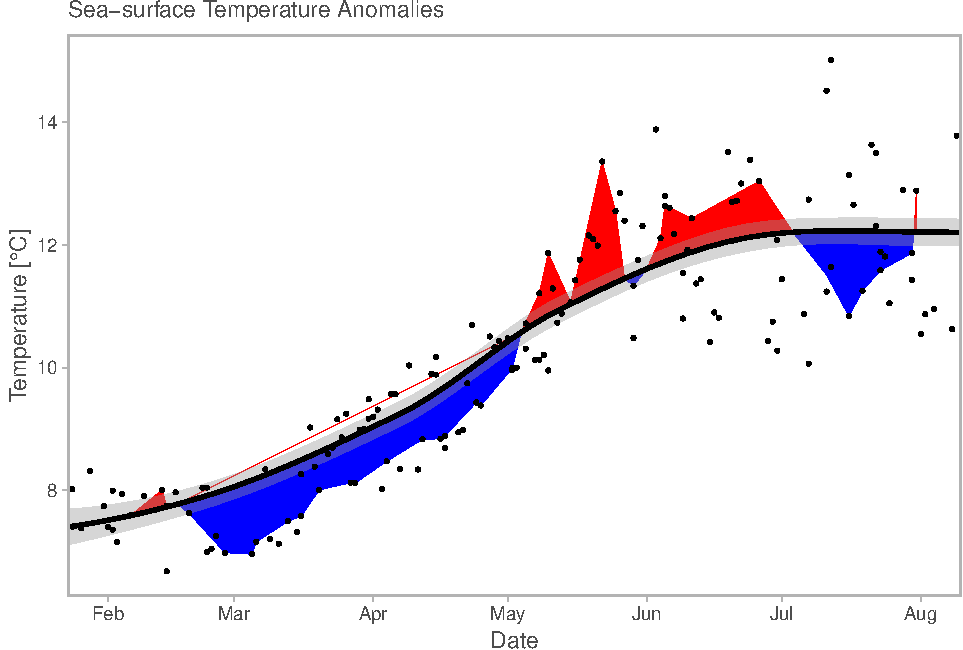
\includegraphics[width=0.9\linewidth]{Migration_Observations_Report_files/figure-latex/sst-1} \caption{Time series of 30 m depth integrated temperature anomalies observed at Hakai Oceanographic Monitoring station QU39. Blue areas represent temperatures that are below average, red areas represent above average temperatures at the selected station in 2018. Average is the solid black line which is a loess regression based on temperatures from 2015-2018. The shaded grey area is 1 SE of the loess regression. The black dots are the daily minimum and maximum temperatures observed over the time series.}\label{fig:sst}
\end{figure}

\section{Tables}\label{tables}

\begin{longtable}[]{@{}rlr@{}}
\caption{\label{tab:z} Key salmon migration health, growth, and migration
parameters standardized to z-scores---the number of standard deviations
observations are from the time series average.}\tabularnewline
\toprule
Year & Parameter & Z-score\tabularnewline
\midrule
\endfirsthead
\toprule
Year & Parameter & Z-score\tabularnewline
\midrule
\endhead
2015 & Sockeye Migration Timing & -0.71\tabularnewline
2016 & Sockeye Migration Timing & 0.00\tabularnewline
2017 & Sockeye Migration Timing & 1.41\tabularnewline
2018 & Sockeye Migration Timing & -0.71\tabularnewline
2015 & Sockeye Catch Intensity & 0.80\tabularnewline
2016 & Sockeye Catch Intensity & 0.93\tabularnewline
2017 & Sockeye Catch Intensity & -0.89\tabularnewline
2018 & Sockeye Catch Intensity & -0.84\tabularnewline
2015 & Sockeye Length & -0.29\tabularnewline
2016 & Sockeye Length & -1.28\tabularnewline
2017 & Sockeye Length & 0.95\tabularnewline
2018 & Sockeye Length & 0.62\tabularnewline
2015 & Sockeye Parasite Loads & 1.40\tabularnewline
2016 & Sockeye Parasite Loads & 0.03\tabularnewline
2017 & Sockeye Parasite Loads & -0.69\tabularnewline
2018 & Sockeye Parasite Loads & -0.75\tabularnewline
2015 & Pink Migration Timing & 1.43\tabularnewline
2016 & Pink Migration Timing & -0.16\tabularnewline
2017 & Pink Migration Timing & -0.89\tabularnewline
2018 & Pink Migration Timing & -0.38\tabularnewline
2015 & Pink Catch Intensity & -0.65\tabularnewline
2016 & Pink Catch Intensity & 0.16\tabularnewline
2017 & Pink Catch Intensity & -0.86\tabularnewline
2018 & Pink Catch Intensity & 1.35\tabularnewline
2015 & Pink Length & 1.30\tabularnewline
2016 & Pink Length & 0.06\tabularnewline
2017 & Pink Length & -0.24\tabularnewline
2018 & Pink Length & -1.12\tabularnewline
2015 & Pink Parasite Loads & 0.77\tabularnewline
2016 & Pink Parasite Loads & -1.23\tabularnewline
2017 & Pink Parasite Loads & 0.86\tabularnewline
2018 & Pink Parasite Loads & -0.40\tabularnewline
2015 & Chum Migration Timing & -1.09\tabularnewline
2016 & Chum Migration Timing & 0.06\tabularnewline
2017 & Chum Migration Timing & 1.32\tabularnewline
2018 & Chum Migration Timing & -0.29\tabularnewline
2015 & Chum Catch Intensity & 0.98\tabularnewline
2016 & Chum Catch Intensity & -1.32\tabularnewline
2017 & Chum Catch Intensity & 0.52\tabularnewline
2018 & Chum Catch Intensity & -0.18\tabularnewline
2015 & Chum Length & 1.41\tabularnewline
2016 & Chum Length & -0.25\tabularnewline
2017 & Chum Length & -0.23\tabularnewline
2018 & Chum Length & -0.94\tabularnewline
2015 & Chum Parasite Loads & 1.03\tabularnewline
2016 & Chum Parasite Loads & -1.37\tabularnewline
2017 & Chum Parasite Loads & 0.22\tabularnewline
2018 & Chum Parasite Loads & 0.12\tabularnewline
2015 & SST & -0.15\tabularnewline
2016 & SST & -0.09\tabularnewline
2017 & SST & -1.09\tabularnewline
2018 & SST & 1.33\tabularnewline
\bottomrule
\end{longtable}

\begin{longtable}[]{@{}llllll@{}}
\caption{\label{tab:mtdi} Migration timing statistics for the cumulative
catch of sockeye, pink, and chum salmon in the Discovery Islands in
2018, compared to the time-series average (2015 - 2018). Q1 is when 25
\% of the species passed through the regions, peak date is the median
when 50 \% passed through, and Q3 is 75\%. The region DI indicates the
Discovery Islands while for species SO is sockeye, PI is pink, and CU is
chum.}\tabularnewline
\toprule
Year & Region & Species & Q1 & Peak Date & Q3\tabularnewline
\midrule
\endfirsthead
\toprule
Year & Region & Species & Q1 & Peak Date & Q3\tabularnewline
\midrule
\endhead
2015 - 2018 & DI & SO & May 26 & May 28 & June 04\tabularnewline
2015 - 2018 & DI & PI & June 07 & June 17 & June 23\tabularnewline
2015 - 2018 & DI & CU & June 06 & June 15 & June 23\tabularnewline
2015 & DI & CU & June 03 & June 05 & June 22\tabularnewline
2015 & DI & PI & June 13 & July 07 & July 07\tabularnewline
2015 & DI & SO & May 23 & May 23 & June 01\tabularnewline
2016 & DI & CU & June 02 & June 15 & June 15\tabularnewline
2016 & DI & PI & June 02 & June 15 & June 15\tabularnewline
2016 & DI & SO & May 24 & May 28 & June 04\tabularnewline
2017 & DI & CU & June 13 & June 26 & July 04\tabularnewline
2017 & DI & PI & June 05 & June 05 & June 26\tabularnewline
2017 & DI & SO & June 05 & June 07 & June 07\tabularnewline
2018 & DI & CU & June 07 & June 12 & June 20\tabularnewline
2018 & DI & PI & June 07 & June 12 & June 12\tabularnewline
2018 & DI & SO & May 23 & May 23 & June 04\tabularnewline
\bottomrule
\end{longtable}

\begin{longtable}[]{@{}rlr@{}}
\caption{\label{tab:catch-intensity} Catch intensity---a measure of inter
annual abundance---for sockeye, pink, and chum in the Discovery Islands
and Johnstone Strait combined.}\tabularnewline
\toprule
Year & Species & Catch Intensity\tabularnewline
\midrule
\endfirsthead
\toprule
Year & Species & Catch Intensity\tabularnewline
\midrule
\endhead
2015 & Sockeye & 355\tabularnewline
2015 & Pink & 50\tabularnewline
2015 & Chum & 377\tabularnewline
2016 & Sockeye & 376\tabularnewline
2016 & Pink & 208\tabularnewline
2016 & Chum & 175\tabularnewline
2017 & Sockeye & 90\tabularnewline
2017 & Pink & 9\tabularnewline
2017 & Chum & 337\tabularnewline
2018 & Sockeye & 99\tabularnewline
2018 & Pink & 438\tabularnewline
2018 & Chum & 275\tabularnewline
\bottomrule
\end{longtable}

\begin{longtable}[]{@{}lllrrl@{}}
\caption{\label{tab:length} Mean fork lengths for each year, species, and
region including the time series average (2015 - 2018), with the 95 \%
confidence interval (95\% CI). The column n indicates the number of fish
measured, except for the time series where n indicates the number of
years averaged.}\tabularnewline
\toprule
Year & Region & Species & n & Fork Length (mm) & 95\% CI\tabularnewline
\midrule
\endfirsthead
\toprule
Year & Region & Species & n & Fork Length (mm) & 95\% CI\tabularnewline
\midrule
\endhead
2015 - 2018 & DI & SO & 4 & 110.9 & 95.9 - 125.9\tabularnewline
2015 - 2018 & DI & PI & 4 & 98.0 & 81.3 - 114.7\tabularnewline
2015 - 2018 & DI & CU & 4 & 105.1 & 91.3 - 118.9\tabularnewline
2015 - 2018 & JS & SO & 4 & 112.5 & 101.2 - 123.8\tabularnewline
2015 - 2018 & JS & PI & 4 & 116.7 & 105.6 - 127.8\tabularnewline
2015 - 2018 & JS & CU & 4 & 118.2 & 110.1 - 126.3\tabularnewline
2015 & DI & SO & 660 & 108.0 & 107.1 - 108.9\tabularnewline
2015 & DI & PI & 56 & 109.6 & 104.9 - 114.3\tabularnewline
2015 & DI & CU & 157 & 117.3 & 114.9 - 119.7\tabularnewline
2015 & JS & SO & 832 & 110.6 & 109.9 - 111.3\tabularnewline
2015 & JS & PI & 105 & 126.9 & 124.8 - 129\tabularnewline
2015 & JS & CU & 134 & 125.4 & 123.5 - 127.3\tabularnewline
2016 & DI & SO & 652 & 99.0 & 98.1 - 99.9\tabularnewline
2016 & DI & PI & 96 & 103.9 & 101.3 - 106.5\tabularnewline
2016 & DI & CU & 124 & 103.3 & 100.7 - 105.9\tabularnewline
2016 & JS & SO & 720 & 103.4 & 102.6 - 104.2\tabularnewline
2016 & JS & PI & 94 & 112.6 & 110.7 - 114.5\tabularnewline
2016 & JS & CU & 104 & 115.0 & 112.9 - 117.1\tabularnewline
2017 & DI & SO & 269 & 120.1 & 118 - 122.2\tabularnewline
2017 & DI & PI & 17 & 90.9 & 82.3 - 99.5\tabularnewline
2017 & DI & CU & 123 & 103.0 & 100.2 - 105.8\tabularnewline
2017 & JS & SO & 181 & 118.8 & 117.2 - 120.4\tabularnewline
2017 & JS & PI & 24 & 115.3 & 112.8 - 117.8\tabularnewline
2017 & JS & CU & 76 & 118.2 & 116 - 120.4\tabularnewline
2018 & DI & SO & 89 & 116.4 & 112.9 - 119.9\tabularnewline
2018 & DI & PI & 229 & 87.4 & 85.8 - 89\tabularnewline
2018 & DI & CU & 211 & 96.7 & 94.6 - 98.8\tabularnewline
2018 & JS & SO & 87 & 117.4 & 113.1 - 121.7\tabularnewline
2018 & JS & PI & 130 & 111.9 & 110.3 - 113.5\tabularnewline
2018 & JS & CU & 130 & 114.3 & 112.7 - 115.9\tabularnewline
\bottomrule
\end{longtable}

\begin{longtable}[]{@{}rrrrrr@{}}
\caption{\label{tab:proptable} The species proportions of total catch in
each year for sockeye, pink, chum, herring, coho, and
Chinook.}\tabularnewline
\toprule
Year & Chum & Coho & Herring & Pink & Sockeye\tabularnewline
\midrule
\endfirsthead
\toprule
Year & Chum & Coho & Herring & Pink & Sockeye\tabularnewline
\midrule
\endhead
2015 & 0.378 & 0.003 & 0.009 & 0.072 & 0.537\tabularnewline
2016 & 0.210 & 0.006 & 0.005 & 0.200 & 0.580\tabularnewline
2017 & 0.661 & 0.018 & 0.008 & 0.012 & 0.301\tabularnewline
2018 & 0.324 & 0.006 & 0.022 & 0.519 & 0.129\tabularnewline
\bottomrule
\end{longtable}

\begin{longtable}[]{@{}lllrlll@{}}
\caption{\label{tab:parasites} Mean sea-lice abundance, prevalence, and
intensity (Margolis et al. 1990) for the time series (2015-2018) as well
as for each species, region, and year with 95\% confidence interval
calculated from annual averages. The region DI indicates the Discovery
Islands and JS Johnstone Strait. Species codes are SO for sockeye, PI
for pink, and CU for chum.}\tabularnewline
\toprule
Year & Region & Species & n & Abundance, 95\% CI & Prevalence, 95\% CI &
Intensity, 95\% CI\tabularnewline
\midrule
\endfirsthead
\toprule
Year & Region & Species & n & Abundance, 95\% CI & Prevalence, 95\% CI &
Intensity, 95\% CI\tabularnewline
\midrule
\endhead
2015 - 2018 & DI & CU & 669 & 0.39 +/- 0.01 & 0.28 +/- 0.01 & 1.41 +/-
0.01\tabularnewline
2015 - 2018 & JS & CU & 469 & 0.48 +/- 0.01 & 0.33 +/- 0.01 & 1.43 +/-
0.01\tabularnewline
2015 - 2018 & DI & PI & 445 & 0.73 +/- 0.06 & 0.38 +/- 0.02 & 1.7 +/-
0.05\tabularnewline
2015 - 2018 & JS & PI & 410 & 0.92 +/- 0.02 & 0.6 +/- 0.01 & 1.55 +/-
0.01\tabularnewline
2015 - 2018 & DI & SO & 1396 & 0.37 +/- 0.01 & 0.26 +/- 0.01 & 1.36 +/-
0.01\tabularnewline
2015 - 2018 & JS & SO & 937 & 0.44 +/- 0.02 & 0.31 +/- 0.01 & 1.38 +/-
0.01\tabularnewline
2015 & DI & CU & 179 & 0.58 +/- 0.14 & 0.4+/-0.33 & 1.44 +/-
0.22\tabularnewline
2015 & DI & PI & 60 & 1.73 +/- 0.4 & 0.72+/-0.59 & 2.42 +/-
0.4\tabularnewline
2015 & DI & SO & 425 & 0.68 +/- 0.09 & 0.43+/-0.38 & 1.58 +/-
0.14\tabularnewline
2015 & JS & CU & 122 & 0.55 +/- 0.15 & 0.37+/-0.28 & 1.49 +/-
0.23\tabularnewline
2015 & JS & PI & 127 & 0.94 +/- 0.18 & 0.57+/-0.48 & 1.64 +/-
0.19\tabularnewline
2015 & JS & SO & 348 & 0.74 +/- 0.11 & 0.46+/-0.4 & 1.63 +/-
0.16\tabularnewline
2016 & DI & CU & 139 & 0.29 +/- 0.13 & 0.19+/-0.13 & 1.52 +/-
0.44\tabularnewline
2016 & DI & PI & 126 & 0.36 +/- 0.13 & 0.24+/-0.17 & 1.5 +/-
0.25\tabularnewline
2016 & DI & SO & 611 & 0.31 +/- 0.05 & 0.23+/-0.2 & 1.37 +/-
0.12\tabularnewline
2016 & JS & CU & 127 & 0.39 +/- 0.15 & 0.28+/-0.21 & 1.36 +/-
0.37\tabularnewline
2016 & JS & PI & 123 & 0.68 +/- 0.15 & 0.49+/-0.4 & 1.4 +/-
0.17\tabularnewline
2016 & JS & SO & 311 & 0.54 +/- 0.1 & 0.35+/-0.3 & 1.53 +/-
0.17\tabularnewline
2017 & DI & CU & 140 & 0.49 +/- 0.15 & 0.34+/-0.26 & 1.42 +/-
0.29\tabularnewline
2017 & DI & PI & 30 & 0.5 +/- 0.32 & 0.33+/-0.17 & 1.5 +/-
0.61\tabularnewline
2017 & DI & SO & 271 & 0.28 +/- 0.07 & 0.22+/-0.17 & 1.25 +/-
0.13\tabularnewline
2017 & JS & CU & 90 & 0.36 +/- 0.14 & 0.27+/-0.18 & 1.33 +/-
0.27\tabularnewline
2017 & JS & PI & 30 & 1.23 +/- 0.35 & 0.77+/-0.58 & 1.61 +/-
0.31\tabularnewline
2017 & JS & SO & 191 & 0.23 +/- 0.07 & 0.2+/-0.14 & 1.16 +/-
0.12\tabularnewline
2018 & DI & CU & 211 & 0.21 +/- 0.07 & 0.17+/-0.12 & 1.25 +/-
0.2\tabularnewline
2018 & DI & PI & 229 & 0.34 +/- 0.09 & 0.25+/-0.19 & 1.37 +/-
0.16\tabularnewline
2018 & DI & SO & 89 & 0.22 +/- 0.11 & 0.18+/-0.11 & 1.25 +/-
0.31\tabularnewline
2018 & JS & CU & 130 & 0.61 +/- 0.17 & 0.4+/-0.32 & 1.52 +/-
0.28\tabularnewline
2018 & JS & PI & 130 & 0.84 +/- 0.17 & 0.55+/-0.46 & 1.54 +/-
0.2\tabularnewline
2018 & JS & SO & 87 & 0.26 +/- 0.11 & 0.22+/-0.14 & 1.21 +/-
0.2\tabularnewline
\bottomrule
\end{longtable}

\begin{longtable}[]{@{}rr@{}}
\caption{\label{tab:ssttable} 30 m depth integrated temperature averages
from May to the end of June in the Northern Strait of Georgia station
QU39.}\tabularnewline
\toprule
Year & Temperature (C)\tabularnewline
\midrule
\endfirsthead
\toprule
Year & Temperature (C)\tabularnewline
\midrule
\endhead
2015 & 11.55\tabularnewline
2016 & 11.56\tabularnewline
2017 & 11.28\tabularnewline
2018 & 11.97\tabularnewline
\bottomrule
\end{longtable}

\section*{References}\label{references}
\addcontentsline{toc}{section}{References}

\hypertarget{refs}{}
\hypertarget{ref-Beamish2001}{}
Beamish, R., and C. Mahnken. 2001. ``A critical size and period
hypothesis to explain natural regulation of salmon abundance and the
linkage to climate and climate change.'' \emph{Progress in Oceanography}
49: 423--37.

\hypertarget{ref-Beamish2012}{}
Beamish, R., C. Neville, R. Sweeting, and K. Lange. 2012. ``The
synchronous failure of juvenile pacific salmon and herring production in
the strait of georgia in 2007 and the poor return of sockeye salmon to
the Fraser river in 2009.'' \emph{Marine and Coastal Fisheries} 4 (1):
403--14.
doi:\href{https://doi.org/10.1080/19425120.2012.676607}{10.1080/19425120.2012.676607}.

\hypertarget{ref-Chandler2017}{}
Chandler, P.C., S.A. King, and J. Boldt. 2017. ``State of the Physical ,
Biological and Selected Fishery Resources of Pacific Canadian Marine
Ecosystems in 2016 Can. Tech. Rep. Fish. Aquat. Sci.'' 3225 (243).
Sidney, BC: Fisheries; Oceans Canada.

\hypertarget{ref-Heard1991}{}
Heard, William R. 1991. ``Life History of Pink Salmon.'' In
\emph{Pacific Salmon Life Histories}, edited by C. Groot and L.
Margolis, 121. 2029 West Mall, Vancouver, BC V6T 1Z2: UBC Press.

\hypertarget{ref-Hunt2018}{}
Hunt, Brian P.V., Brett T. Johnson, Sean C. Godwin, Martin Krkošek,
Evgeny A Pakhomov, and Luke A Rogers. 2018. ``The Hakai Institute
Juvenile Salmon Program : Early Life History Drivers of Marine Survival
in Sockeye , Pink and Chum Salmon in British Columbia.'' Institute for
the Oceans; Fisheries; Department of Earth, Ocean; Atmospheric Sciences,
University of British Columbia, Hakai Institute, Earth to Ocean Research
Group, Simon Fraser University, Department of Ecology; Evolutionary
Biology, Univer.

\hypertarget{ref-Margolis1990}{}
Margolis, L., G. W. Esch, A.M. Kuris, and G.A. Schad. 1990. ``The Use of
Ecological Terms in Parasitology (Report of an Ad Hoc Committee of the
American Society of Parasitologists).'' \emph{The Journal of
Parisitology} 68 (1): 131--33.
doi:\href{https://doi.org/10.2307/3281335}{10.2307/3281335}.

\hypertarget{ref-Patanasatienkul2013}{}
Patanasatienkul, Thitiwan, Javier Sanchez, Erin E. Rees, Martin Krkošek,
Simon R.M. Jones, and Crawford W. Revie. 2013. ``Sea lice infestations
on juvenile chum and pink salmon in the Broughton Archipelago, Canada,
from 2003 to 2012.'' \emph{Diseases of Aquatic Organisms} 105 (2):
149--61. doi:\href{https://doi.org/10.3354/dao02616}{10.3354/dao02616}.

\hypertarget{ref-Peterman2010}{}
Peterman, Randall M, D Marmorek, B Beckman, M Bradford, M Lapointe, N
Mantua, Brian Riddell, et al. 2010. ``Synthesis of evidence from a
workshop on the decline of Fraser River sockeye. June 15-17, 2010. A
Report to the Pacific Salmon Commission.'' August. Vancovuer, British
Columbia: Pacific Salmon Commission.

\hypertarget{ref-R}{}
R Core Team. 2017. \emph{R: A Language and Environment for Statistical
Computing}. Vienna, Austria: R Foundation for Statistical Computing.
\url{https://www.R-project.org/}.



\end{document}
